\section{Implementation}

\subsection{Linear-logarithmic pixel}

The primary design idea is the linear-logarithmic APS, using a threshold voltage to switch between the 
two operation modes automatically \cite{withTable, withCompensation}. It is based on a \(3T\) pixel,
with an additional photodiode used to compensate the current of the primary detector. In this particular case,
the threshold will be variable based on the output, instead of being set to a fixed value for the entire operation.

\begin{figure}[H]
    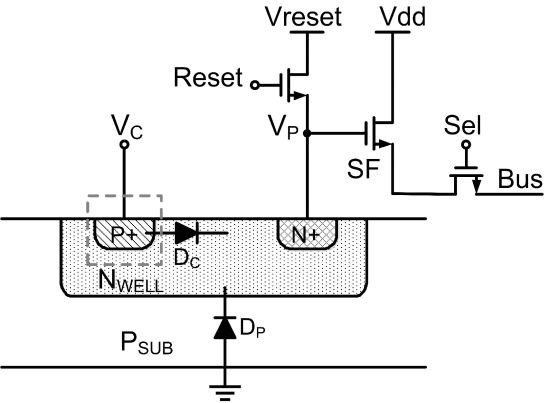
\includegraphics[width=0.50\textwidth, height=0.45\textwidth]{resources/png/secondCircuit.png}
    \caption{Pixel schematic. \cite{withCompensation} \label{figPixel}}
\end{figure}

In \ref{figPixel}, photodiode \(D_{C}\) is connected to the voltage source, \(V_{C}\), as well as the other
photodiode, \(D_{P}\). It acts as a switch, based on \(V_{C}\) and the current illumination. In low light conditions,
the \(D_{C}\) is reverse biased and the potential in point \(V_{P}\) is higher than \(V_{C}\). In this case,
the output voltage increases linearly with the illumination and integration time:

\begin{equation}
    \label{eqLinOutput}
    V_{out-lin} = V_{DD} - {t_{int}I_{P}}
\end{equation}

with \(t_{int}\) the integration time and \(I_{P}\) the current provided by \(D_{P}\).

For higher illumination or integration time, \(D_{C}\) becomes forward biased and compensates the voltage of \(D_{P}\),
with the potential in \(V_{P}\) falling under \(V_{C}\). In this case, the output is no longer linear, but logarithmic:

\begin{equation}
    \label{eqLogOutput}
    V_{out-log} = V_{C} - V_{T}\ln{\frac{I_{P}}{I_{S}}}
\end{equation}

with \(I_{S}\) denoting the saturation current provided by \(D_{c}\), and \(V_{T}\) denoting the thermal voltage. 

In logarithmic mode, there is potential for significantly higher amounts of fixed pattern noise (FPN). This issue
is mitigated by \cite{withTable} by introducing a two-step charge transfer. This process however introduces and additional
gate for signaling when each readout is triggered. The current Implementation aims to resolve the noise issue by
allowing each pixel to reduce the threshold voltage based on previous outputs.

\subsection{Individual threholding}

Similar to the feedback loop in time variant APS systems \cite{withTime}, this implementation uses a feedback loop
in order to change the cutoff point between linear and logarithmic outputs. Based on the results of \cite{withTable, withCompensation},
the optimal threshold value, obtaining a dynamic range of \(168dB\), is \(1.5V\). This approach however, leads
to significant amounts of the output being computed in the logarithmic domain. 

In order to circumvent the aforementioned issue, the current approach makes use of the relation between the threshold
voltage and the cutoff intensity, being that the switch-off happens at lower illumination values as \(V_{C}\) increases.

\begin{figure}[H]
    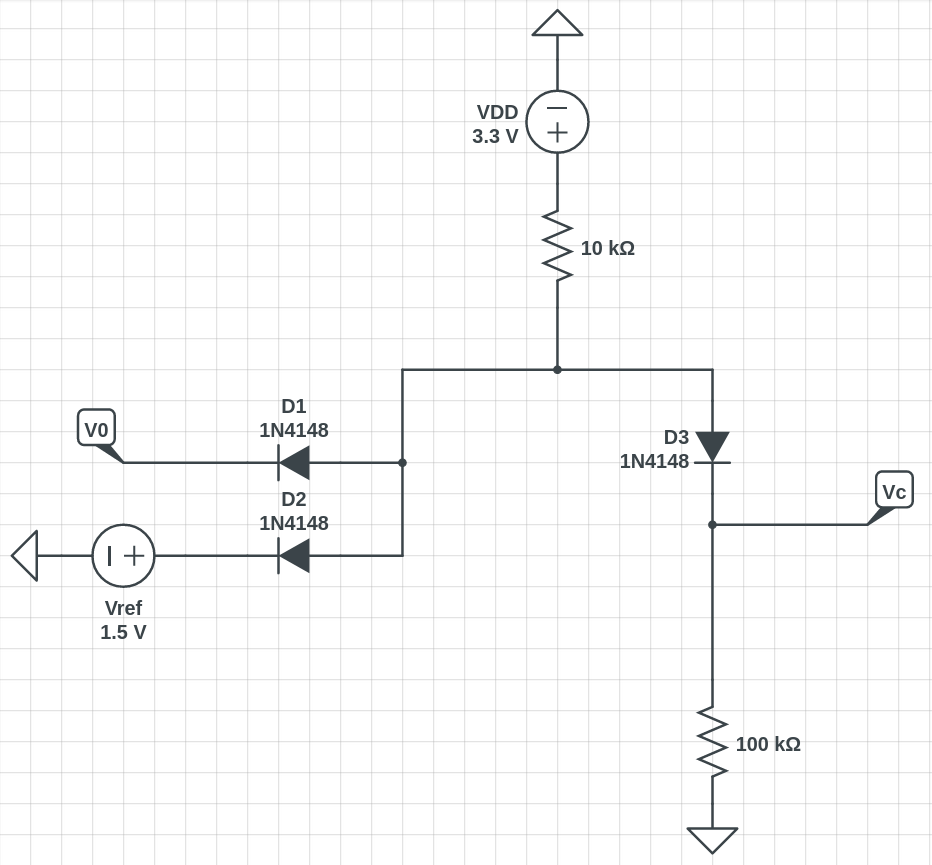
\includegraphics[width=0.50\textwidth, height=0.55\textwidth]{resources/png/minimum.png}
    \caption{Feedback loop. \label{figFeedback}}
\end{figure}

Showcased in \ref{figFeedback} is the feedback loop, a minimizing circuit meant to set

\begin{equation}
    \label{eqFeedback}
    V_{C} = \min(V_{out}, V_{ref})
\end{equation}

with the reference voltage \(V_{ref}\) set to the aforementioned \(1.5V\). This ensures that, if the output surpasses \(1.5V\),
the threshold voltage will remain at the level that allows for best performance. In all other cases, if lower illumination
levels are detected for an individual pixel, the specific DR is reduces, allowing more information to be 
passed as a linear response.
